
%%%%%%%%%%%%%%%%%%%%%
\chapter{Définitions}
%%%%%%%%%%%%%%%%%%%%%


\begin{itemize}[leftmargin=1.7cm, label=\ding{32}, itemsep=5pt]%\end{itemize}
\item  {\bf Case faible} : case qui ne peut plus être contrôler par un pion.
\item  {\bf Colonne fermée} : des pions l'obstruent.
\item  {\bf Colonne ouverte} : il n'y a plus de pion dessus.
\item  {\bf Colonne semi-ouverte} : Il y a un pion dessus.
\item  {\bf Faiblesses} : pion arriéré, pion isolé, pièce non protégée,...
\item  {\bf Finales} : commence après l'échange des dames.
\item  {\bf Milieu} : entre l'ouverture et la finale. 
\item  {\bf Ouverture} : début de la partie, se termine avec la liaison des tours.
\item  {\bf Pion arriéré} : pion ne pouvant être défendu aisément par un pion.
\item  {\bf Pions doublés} : pions du même joueur sur une même colonne.
\item  {\bf Pion isolé} : pion ne pouvant plus être défendu par un pion.
\item  {\bf Position fermée} : Les colonnes sont fermées.
\item  {\bf Position ouverte} : Des colonnes sont ouvertes ou semi-ouvertes.
\end{itemize}
%\begin{itemize}[leftmargin=1cm, label=\ding{32}, itemsep=1pt]
%\item {\bf } : \end{itemize}

\vfill

\begin{center}
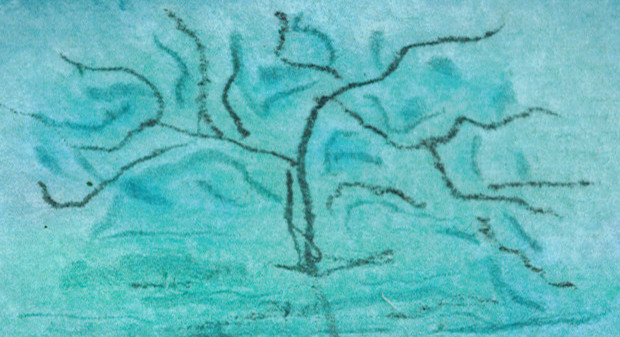
\includegraphics[scale=2.1]{./image/arbre}
\end{center}

\vfill

%%%%%%%%%%%%%%%%%%%%%%%%%%%%%%%%%%%%%%%%%%%%%%%%%%%%%%%
